%=================================================================
%				preamble
%=================================================================
\documentclass[11pt,letterpaper]{book}

\newcommand{\theauthor}{Thomas Graf}		        
\newcommand{\university}{Stony Brook University}	
\newcommand{\emailaddress}{lin637@thomasgraf.net}
\newcommand{\coursenumber}{Lin637}
\newcommand{\coursename}{Computational Linguistics 2}
\newcommand{\thetitle}{\texorpdfstring{\coursenumber\\ \coursename}{\coursenumber --- \coursename}}
\newcommand{\thekeywords}{graduate level, lecture, computational linguistics, phonology, syntax}
\newcommand{\thedate}{}

\usepackage{mypackages}
\usepackage{mycommands}



%=================================================================
%			title format
%=================================================================
\author{\theauthor}
\title{\thetitle}
\date{\thedate}

%=================================================================
%			content
%=================================================================
% \includeonly{./tex/ConstituencyTests}

\begin{document}
\raggedbottom
\pagenumbering{Roman}
\maketitle
\tableofcontents
\clearpage

\setcounter{chapter}{-1}
\chapter{Syllabus}
\label{cha:syllabus}
\setcounter{page}{1}

\fcolorbox{gray!25}{gray!25}{%
    \centering
    \begin{tabular}{ll}
        \textbf{Course:} Computational Linguistics 2&
        \textbf{Name:} Thomas Graf\\
        \textbf{Course\#:} Lin637 &
        \textbf{Email:} \href{mailto:lin637@thomasgraf.net}{lin637@thomasgraf.net}\\
        \textbf{Time:} TR 10:00--11:20am &
        \textbf{Office hours:} tba \\
        \textbf{Location:} Humanities 2047 &
        \textbf{Office:} SBS N249\\
        \textbf{Course Website:} \href{http://lin637.thomasgraf.net} {lin637.thomasgraf.net} &
        \textbf{Personal Website:} \href{http://thomasgraf.net}{thomasgraf.net}
    \end{tabular}
}

\section{Course Outline}

\subsection{Bulletin Description}
An introduction to the theoretical foundation of computational linguistics.
The course emphasizes the importance of algorithms, algebra, logic, and formal language theory in the development of new tools and software applications.
Empirical phenomena in phonology and syntax are sampled from a variety of languages to motivate and illustrate the use of concepts such as strictly local string languages, tree transducers, and semirings.
Students will develop familiarity with the literature and tools of the field.

\subsection{Full Description}

This course serves a specific purpose in our program (see Fig.~\vref{fig:Syllabus_Program}):
it acts as the bridge from introductory courses in linguistics (Syntax 1, Phonology 1, Phonetics) and computational methods (Statistics, Mathematical Methods in Linguistics, Computational Linguistics 1) to advanced courses and seminars in computational\slash mathematical linguistics.
In contrast to the NLP courses offered by the department of computer science, our courses focus on studying the properties of natural language from a computationally informed perspective.
The question is not how computers can solve linguistic tasks, but how language can be conceptualized as a computational problem.
This emphasis is also reflected in the selection of topics for this course.

\begin{itemize}
    \item \textbf{What this course is not about}
        \begin{itemize}
            \item Computer-assisted research methods in linguistics
            \item Programming
            \item Software development for natural language tasks
        \end{itemize}
    \item \textbf{What is not covered but benefits from what is covered}
        \begin{itemize}
            \item Speech recognition
            \item OCR
            \item Text generation
            \item Parsing
            \item Semantic analysis
            \item Machine translation
        \end{itemize}
    \item \textbf{List of topics}
        \begin{itemize}
            \item \emph{Phonology and Morphology}
                \begin{itemize}
                    \item The role of formalization
                    \item String languages
                    \item Subregular hierarchy
                    \item Regular languages
                    \item Generative capacity of phonology
                    \item String transductions
                    \item 2-level morphology
                    \item Equivalence of SPE and OT
                \end{itemize}
            \item \emph{Syntax}
                \begin{itemize}
                    \item Tree languages
                    \item Syntax is more complex than phonology
                    \item Mildly context-sensitive formalisms (TAG, MGs)
                    \item Tree transductions
                    \item Regular representations of MCS formalisms
                    \item Reinterpreting the T-model
                \end{itemize}
        \end{itemize}
\end{itemize}

A rough outline of the course progression is given in Tab.~\vref{tab:Syllabus_CourseOutline}.
Many of the topics we cover draw from very specialized areas of formal language theory that even most mathematicians and computer scientists do not know about, e.g.\ the correspondence between finite-state machines and monadic second-order logic, or the logical characterization of tree transductions.
So this course might be of value to you even if you do not particularly care about natural language.
Make no mistake, though, we'll talk a lot about language and linguistics --- this is not a math class.

\begin{table}
    \centering
    \begin{tabular}{rp{5.5cm}p{5.5cm}}
        \toprule
        \emph{Wk} & \emph{Formal} & \emph{Linguistics} \\
        \toprule
        1         & What is computation? & Marr's Three Levels\\
        2         & Formalizing phonology & Why formalize?\\
        3         & Strictly local languages & Local dependencies\\
        4         & Subregular hierarchy & How powerful is phonology?\\
        5         & Regular languages & Abstractness\\
        6         & String transductions & SPE-OT equivalence\\
        7         & Two-level morphology & Null morphemes\\
        \midrule
        8         & (Spring Break) & \\
        \midrule
        9         &  Weak Generative Capacity & $\text{Phonology} < \text{Syntax}$\\
        10        &  Tree languages & Headedness, feature percolation\\
        11        &  Local tree languages & GPSG\\
        12        &  Recognizable tree languages & GB\\
        13        &  TAG and MGs & Minimalist syntax\\
        14        &  Tree transductions & Reinterpreting the T-model\\
        15        &  Unification via first-order logic & Strictly Derivational Minimalism\\
        \bottomrule
    \end{tabular}
\caption{Tentative course outline}
\label{tab:Syllabus_CourseOutline}
\end{table}

\begin{figure}
    \rotatebox{0}{
        \footnotesize
        \begin{tikzpicture}[
    every node/.style = { draw, thick },
    every path/.style = { ->, thick },
    sug/.style = { dashed },
    req/.style = { },
    ]
    \node (CL2) at (0,0) [align=center] {Computational Linguistics 2\\ (Lin 637)};

    % Prereqs
    \node (Phon) [above=of CL2, xshift=-8em, align=center] {Phonology 1 (Lin 522)\\
                                                                \emph{or}\\
                                                            Phonetics (Lin 523)
                                                        };
    \node (Syntax) [left=of Phon, align=center] {Syntax 1\\ (Lin 521)};
    \node (Math)   [above=of CL2, xshift=8em, align=center] {Statistics (Lin 538)\\
                                                                \emph{or}\\
                                                            Mathematical Methods (Lin 539)
                                                        };
    \node (CL1) [right=of Math, align=center] {CompLing 1\\ (Lin 537)};

    % CS branch
    \node (NLP) [below right=of CL2, xshift= 8em, align=center] {Introduction to NLP\\ (CSE 628)};
    \node (Machine) [below=of NLP, xshift=-8em, align=center]  {Machine Learning\\ (CSE 512)};
    \node (Speech)  [below=of NLP, xshift= 8em, align=center] {Speech Processing\\ (CSE 542)};

    % Linguistics branch
    \node (CompSem) [below=of CL2, xshift=-16em, align=center] {Computational Semantics\\ (Lin 626)};
    \node (CompPhon) [below=of CompSem, align=center] {Computational Phonology\\ (Lin 627)};
    \node (CompSyn) [below=of CompPhon, align=center] {Computational Syntax\\ (Lin 628)};

    \node (Learn) [right=of CompSem, xshift=4em, align=center]  {Learnability\\ (Lin 629)};
    \node (Parse) [right=of CompPhon, xshift=4em, align=center] {Parsing and Processing\\ (Lin 630)};

    % Branches
    \draw[sug] (Syntax) |- (CL2);
    \draw[sug] (Phon) to (CL2);
    \draw[sug] (Math) to (CL2);
    \draw[req] (CL1) |- (CL2);
    \draw[req] (CL1.south -| NLP.north) -- (NLP);
    \draw[sug] (NLP) -| (Machine);
    \draw[sug] (NLP) -| (Speech);
    \draw[sug] (Learn |- CL2.south) -- (Learn); 
    \draw[sug, transform canvas={xshift=2em}] (Parse |- CL2.south) -- (Parse);
    \draw[sug] ($(CL2.south)-(6em,0)$) |- (CompSem);
    \draw[sug] ($(CL2.south)-(5em,0)$) |- (CompPhon);
    \draw[sug] ($(CL2.south)-(4em,0)$) |- (CompSyn);
\end{tikzpicture}

    }
\caption{Computational Linguistics 2 in the curriculum (dashed lines indicate recommendations rather than prerequisites)}
\label{fig:Syllabus_Program}
\end{figure}    

\subsection{Prerequisites}

The only official prerequisite is Computational Linguistics 1 (Lin 537) or comparable programming skills in Python.
Python will be used to illustrate some formal concepts, and some of the homeworks will require you to implement an algorithm or procedure in Python.
Prior experience with git, markdown, and \LaTeX\ is useful for the homeworks but not required.

It is also helpful to have some basic familiarity with linguistics (phonemes, phrase structure rules, syntactic trees) and mathematics (sets, functions, relations, and first-order logic as covered in Semantics 1, for instance).
You can take an online survey to identify weaknesses, and several introductory readings on these topics are available on the course website.

\medskip
\noindent
\hspace{-.75em}
\begin{tabular}{ll}
    \textbf{Survey URL:} & 
    \href{https://testmoz.com/432409}{https://testmoz.com/432409}\\
    \textbf{Password (if required):} &
    CompLing2
\end{tabular}

\section{Teaching Goals}
\begin{itemize}
    \item \textbf{Practical Skills}
        \begin{itemize}
            \item conceptualize a problem in mathematical terms
            \item optimize your programs through the use of adequate algorithms and data structures (dynamic programming techniques, hash tables, etc.)
            \item a more abstract and theoretically informed perspective on current tools and techniques in NLP
            \item an understanding for how linguistic insights can be invoked to simplify NLP tasks
        \end{itemize}
    \item \textbf{Research Skills}
        \begin{itemize}
            \item assess linguistic phenomena from a computational perspective
            \item evaluate linguists' claims about computational efficiency
            \item basic overview of current research in theoretical computational linguistics
            \item use computational concepts to identify new empirical generalizations
            \item bring linguistic data to bear on computational claims
            \item mathematically informed understanding of linguistic theories
        \end{itemize}
\end{itemize}


\section{Grading}
\begin{itemize}
    \item \textbf{Homework}
        \begin{itemize}
            \item weekly exercises, programming assignments, or critical evaluations of assigned readings
            \item Homework submission and grading is done via github.
            \item No late hand-ins!
            \item Collaboration on homework problems is encouraged as long as you write up the solutions by yourself, using your own words, examples, notation, and code.
        \end{itemize}
        %
    \item \textbf{Readings}
        \begin{itemize}
            \item about two readings per week
            \item you have to collaboratively write a summary for each reading in the course wiki
        \end{itemize}
        %
    \item \textbf{Survey Squibs}
        \begin{itemize}
            \item By the end of the course, the wiki should contain survey articles on a number of topics not covered in this course (or not covered at the same depth).
            \item You have to pick a topic and write the corresponding survey article.
            \item These articles should be succinct and simple enough that they are comprehensible to a researcher with little exposure to computational linguistics, yet at the same time include enough technical detail that the claims can be verified by somebody with the appropriate background.
                (Why this weird requirement?
                Because that's the recipe for writing a computational paper that can be published in a linguistics journal!)
        \end{itemize}
        %
    \item \textbf{Workload per Credits}
        \begin{itemize}
            \item \emph{3 credits}: homework, readings, squib
            \item \emph{2 credits}: homework, readings
            \item \emph{1 credit}: readings
            \item \emph{0 credits}: none, but I highly recommend that you at least read the assigned papers as they will be important for following the lectures
        \end{itemize}
\end{itemize}


\section{Online Component}

This class uses some online tools to facilitate homework collaboration and submission, student discussions, and dynamic lecture evaluation.

\begin{itemize}
    \item \textbf{Homework submission}\\
        \emph{How it works:}
        Homeworks will distributed via a github repository. 
        You can fork this repo and upload your own code, or checkout other students' forks to see how they dealt with the problem.
        In order to submit a homework you upload your solution to your fork and issue a pull request.
        After the due date, I'll upload my solution to the repository.

        \emph{Why we do it:}
        This setup mimics the modern workflow in collaborative development projects.
        Git is one of the best-known version control systems, and github is the biggest online service for hosting git repositories.
        Familiarity with version control systems is an essential job requirement for computational linguists, and it is also very helpful for academic work.
        See this discussion on Stackflow for some ideas how git can be used in conjunction with Latex:
        \href{http://stackoverflow.com/questions/6188780/git-latex-workflow}{http://stackoverflow.com/questions/6188780/git-latex-workflow}

        \emph{What you'll need:}
        A github account (the free tier is enough) and a way of uploading your code to a github repository. Linux users can install git via the command line, whereas Windows and Mac users should download and install the github app, which comes with a nice GUI.

    \item \textbf{Homework Feedback and Discussion}\\
        \emph{How it works:}
        Every github repository comes with an issue (= ticket) tracker.
        If you have a question or wish to discuss a topic, you can open a ticket on the main repository (note: tickets support markdown).
        I may also use tickets to leave comments on your homeworks.

        \emph{Why we do it:}
        Once again this is an essential part of modern software development.
        And it is also a lot more convenient than anything Blackboard has to offer.

        \emph{What you'll need:}
        Not much beyond the ability to navigate the github repos.

    \item \textbf{Reading summaries}\\
        \emph{How it works:}
        Every week I create an empty page on the course wiki for each assigned reading.
        Your job is to expand these articles into useful summaries.
        The default syntax for the wiki entries is markdown, a very simple \emph{lingua franca} for writing plain text documents that can easily be converted into a variety of file formats (doc, pdf, html, and so on).

        \emph{Why we do it:}
        Wikis are frequently used for software documentation nowadays, so you have to know how to work with one.
        You will also get to see the advantages of markdown, in particular for short documents that do not need a lot of fancy typesetting (this can even include your own website!).
        Hopefully this will move you away from formats like doc, which
        %
        \begin{itemize*}
            \item are proprietary, and
            \item lack backwards compatibility, and
            \item are tedious to index and search, and
            \item fail to separate the content of a document from its presentation, thereby distracting you with unnecessary details.
        \end{itemize*}
        %
        Also, learning markdown takes a lot less time than relearning the MS Office user interface with each new version.
        If you find that markdown is too simple for your own purposes, you can also switch to a more expressive superset like \href{http://johnmacfarlane.net/pandoc/}{pandoc}.

        \emph{What you'll need:}
        Nothing except the ability to read (and ideally write in) markdown.
        The github editor makes this fairly easy with its built-in help, formatting buttons and dynamic preview.
        You can also checkout this interactive markdown tutorial, which should take you about 15 minutes (yes, markdown is that easy!):
        \href{http://markdowntutorial.com/}{http://markdowntutorial.com/}

    \item \textbf{Class announcements}\\
        \emph{How it works:}
        Normal announcements (readings, due dates) are put on the course website, time-critical ones (i.e.\ class cancellations) are emailed out via Blackboard.
        
        \emph{What you'll need:}
        If you're not officially enrolled in the course, send me a message so I can add you to Blackboard.

    \item \textbf{Handouts}\\
        \emph{How it works:}
        Handouts are made available online Monday and Wednesday before 3pm.
        You can look at them on your laptop\slash tablet or make a hardcopy before class.
        I will not bring handouts to class unless I could not upload them on time the day before.

        \emph{Why we do it:}
        Mostly because I just don't like paper.
        Also keep in mind that you can fork the lecture notes repository and include your notes directly in the Latex source files.
        Then you can compile a version of the lecture notes with your own notes already included.
\end{itemize}


\section{Policies}

\subsection{Contacting me}
\begin{itemize}
    \item Emails should be sent to \href{mailto://lin637@thomasgraf.net}{lin637@thomasgraf.net} to make sure they go to my high priority inbox.
        Disregarding this policy means late replies and is a sure-fire way to get on my bad side.
    \item Reply time < 24h in simple cases, possibly more if meddling with bureaucracy is involved.
    \item If you want to come to my office hours and anticipate a longer meeting, please email me so that we can set apart enough time and avoid collisions with other students.
\end{itemize}

\input{./tex/blabla.tex}


\pagenumbering{arabic}

\chapter{Implementing Phonology as a List}
\label{cha:ListPhonology}

Word-final devoicing is a very common process which turns voiced consonants (\textipa{/b/}, \textipa{/d/}, \textipa{/g/}, \textipa{/z/}, \ldots) that occur at the end of a word into their voiceless counterparts (\textipa{/p/}, \textipa{/t/}, \textipa{/k/}, \textipa{/s/}, \ldots).
It usually applies only to a proper subclass of a given language's full inventory of voiced sounds.
Final devoicing is attested in a rich variety of languages, from Indo-European ones like Catalan (Romance), German (Germanic), and Russian (Slavic) to Turkish (Turkic, Altaic) and Wolof (Senegambian, Niger-Congo).

\begin{center}
    \begin{tabular}{r@{\hskip 4em}ll}
        \toprule
        \textbf{Language} & \textbf{Voiced} & \textbf{Devoiced}\\
        \toprule
        Catalan & \emph{grize} `gray (\gloss{f})' & \emph{gris} `gray (\gloss{m})'\\
        German & \emph{räder} `bikes' & \emph{rat} `bike'\\
        Russian & \emph{kniga} `book (\gloss{Nom.Sg.}) & \emph{knik} `book (\gloss{Gen.Pl.})'\\
        Turkish & \emph{sarabi} `wine (\gloss{Acc.Sg.})' & \emph{sarap} `wine (\gloss{Nom.Sg.})'\\
        Wolof &  does anybody know & the data?\\
        \bottomrule
    \end{tabular}
\end{center}

What kind of computational resources must a native speaker possess that has successfully learned this process for their language and can apply it correctly during speech?
As innocent as this question may seem, it is actually very difficult to answer because it is unclear what the process of word-final devoicing is.

The way it was described above --- which is the standard view among phonologists --- it is a process that takes a word as an input and returns an output where any word-final voiced consonants have been devoiced.
That is a complex idea that involves three distinct components:
%
\begin{enumerate*}
    \item an input form,
    \item an output form,
    \item a process translating the former into the latter.
\end{enumerate*}
%
It is far from obvious that this is indeed what speakers are doing; all we can tell for sure is that speakers produce the correct output forms.
So rather than jumping immediately into the deep waters of sophisticated phonological machinery, let's see what the \textbf{simplest empirically adequate} solution might be.
It might well turn out that speakers are actually doing something more complicated, but at least we will have a better understanding of the problem and a computational baseline that we can compare speakers' behavior to.


\section{The Simplest Model: Phonology as a List}

Arguably the simplest conceivable solution is that there are no phonological processes at all, speakers simply memorize all the output forms.
This would reduce phonology to a long list of fully inflected words and speakers simply pick that item from the list that they want to pronounce.
It explains speakers' ability to produce the correct output form purely via memorization, no computational machinery is required beyond a mechanism for storing and retrieving phonetic strings. 
Such a solution is certainly simple, but is it empirically adequate?

\subsection{Storage and Retrieval Speed of Lists}

Let's first think about whether speakers could possibly have such a list stored somewhere in their brain.
Psychologists and neuroscientists still know very little about how the brain stores information, so for the sake of argument we will look at this through the lens of Python data structures.
Python has lists as a data type, so we could instantiate a phonology list for a given language, say German:
%
%fixme: margins

\begin{pythoncode}
    german_phonology = ['rat', 'r"ada', 'blint', 'blinde',\
                        'ich', 'du', 'ea', 'sii', 'Es']
\end{pythoncode}
%fixme: add comment about notation
%
The problem is that items in a list are not readily accessible.
If you know the index of an item, you can readily access it as below.

\begin{pythoncode}
    german_phonology[4]
\end{pythoncode}
%
But with long lists you do not know which position a specific item occupies.
In order to retrieve this item, then, one has to search through the entire list until one finds the correct item.
So the longer the list, the longer it takes to find an item towards its end.
If we simply search through the list from left to right, finding the $n$-th item takes $n$ steps.

%fixme: add part about BigO notation

This does not seem at all plausible from a psycholinguistic perspective.
Experiments have shown that frequent words are retrieved more quickly than rarer ones, but % fixme: expand how we don't see linear search, add references

\subsection{Hash Tables and Python Dictionaries}

Quick access and storage of information is crucial in various applications, and thus it is no surprise that computer scientists have developed data structures which allow any given item to be stored and retrieved in constant time.
A particularly popular one is the \emph{hash table}.
The basic idea behind a hash table is that the problem with lists is the arbitrary and volatile connection between an item in a list and its index.
Not only is there no particular reason why \emph{blint} has index $2$ and \emph{ea} index $1$, their indices can also change, e.g. if elements are added to the list or if the entries in the list are reordered.
In a hash table, each entry has a key that uniquely identifies it, and this key is translated into the correct index via a \emph{hash function}.
Hence the order of elements in a hash table is irrelevant for their retrieval.
As long as we have the key, lookup takes only the amount of time required to compute the index from the key.
A smart hash function can do this in constant time for any given key irrespective of how many keys there are or how long they are --- the conversion from indices to keys always takes a fixed number of steps.
It follows that lookup in hash table takes constant time, much more efficient than the linear time lookup in a list.
%fixme: hash tables are more complicated
%fixme: add O(1)

Python dictionaries are an implementation of hash tables, so we can improve the performance of our list implementation simply by switching to a different data structure.
That requires only minor changes in the code.
First, we change to curly braces to signal that we are constructing a dictionary.
Then each item is assigned a unique key, for which we choose the underlying form posited by phonologists.

\begin{pythoncode}
    german_phonology = {'rad':'rat', 'r"ader':'r"ada',\
                        'blind':'blint', 'blinde':'blinde',\
                        'ich':'ich', 'du':'du', 'er':'ea',\
                        'sii':'sii', 'Es':'Es'}
\end{pythoncode}

But now that lookup is constant time thanks to the use of a dictionary we outperform the psycholinguistic reality that not all words are equally easy to retrieve.
It is conceivable, though, that humans use a hash function that prioritizes quick retrieval of common items to the detriment of less frequent ones.
After all, a hash function that takes one step on very frequent items and five steps on rare ones might be preferable to one that takes 3 steps for all of them.
From the perspective of computational complexity the two are the same because $\BigO(1) = \BigO(3) = \BigO(5)$, but that does not preclude that one is noticeably faster than the other in practice, at least when run on \emph{wetware}, i.e.\ the human brain.
Or maybe frequent words are stored in a faster type of memory (just like you might have your OS installed on an SSD while keeping your media files on a conventional hard drive).
So let's graciously assume that this aspect of human performance can be modeled (and possibly explained) by the phonology list approach.

\subsection{Memory Usage}

The next question one might ask is whether it is feasible that humans do indeed store all words in their fully inflected forms.
Remember that this is a crucial assumption for the model under discussion, which treats phonology as nothing more than an inventory of the well-formed outputs.
We can do some rough estimates regarding memory usage.

Let's make the conservative estimate that the speaker's language has 30 different allophones. 
So each sound in a word can be represented by a number between 0 and 29.
For instance, \emph{rad} may correspond to \emph{21 5 13}.
How many bits does it take to store one of these numbers?
Since a bit can be either $0$ or $1$, the number of bits is exactly the number of digits used in the binary representation. 
The highest number we need is $29$, which is represented as 11011 in binary, so each number (= sound) requires at most $5$ bits.
We will take $4$ as the average (assuming that some sounds are more common than others, a smart coding strategy could push this down quite a bit).
We furthermore assume that the speaker's vocabulary contains about 20,000 words, which expands to about 50,000 fully inflected word forms, with an average word length of $8$.
Hence we have 50,000 words that take $8 \cdot 4$ bits on average.
Overall then, we need $\frac{50000 \cdot 8 \cdot 4}{8 \cdot 1024} \approx 196 $ Kilobytes to store all these forms.
To put this number into perspective, the collected works of Shakespeare take up about 20 times as much (2 to 5 Megabytes depending on character encoding) and fits on 1500 densely printed pages.
The phonology list model, then, would take up about 75 pages, which doesn't seem to outrageous --- humans are certainly capable of memorizing longer passages. 
%fixme: remark about indian oral tradition

Things do not get much worse as the number of allophones increases.
Some languages like Ubyx have over 70 allophones for consonants alone.
In this case, we may need number ranges between 0 and 80 or even higher, which implies an increase in the maximum number of bits per sound to 7, so with an average of 6 bits we would end up using 292 Kilobytes, or 111 pages.

\subsection{Prefix Trees}

Notice that these are only the storage requirements for the output forms, not for the keys and the (negligible) hash function.
With no further optimizations, the keys will double the memory usage.
The keys we use, though, have the property that many of them are very similar.
For instance, the keys \emph{blind} and \emph{blinde} are almost exactly the same.
The latter is an extension of the former, or the other way round, \emph{blind} is a \emph{prefix} of \emph{blinde}.
%
\begin{definition}[Prefix]
    Given strings $u$ and $w$, $u$ is a \emph{prefix} of $w$ iff there is some (possibly empty) string $v$ such that $w$ is the concatenation of $u$ and $v$.
\end{definition}
%
Keep in mind that this usage of prefix has nothing to do with its linguistic meaning as an affix that precedes the stem of a word.
Furthermore, since $v$ in the definition is allowed to be empty, i.e.\ a string that contains no symbols whatsoever, every string is its own prefix.
For instance, the prefixes of \emph{blinde} are \emph{b}, \emph{bl}, \emph{bli}, \emph{blin}, \emph{blind}, and \emph{blinde} itself.

Considering that morphology in many languages relies on suffixes, it is very likely that the keys in the phonology list of a given language show a great amount of overlap.
This allows us to represent them in a more memory-efficient way via a \emph{prefix tree} (also called \emph{trie}) like the one below.
%
\begin{center}
    \begin{tikzpicture}[
    state/.style = {circle, fill=blue!15, inner sep = 0pt, minimum width = 2em},
    final/.style = {circle, fill=red!15, inner sep = 0pt, minimum width= 2em},
    keylabel/.style = {black},
    arc/.style = {->,gray!75}
    ]
    
    \node[state] (root) at (0,0) {};

    \node[state] (b) [xshift=-13em,below=of root] {};
    \node[state] (d) [right=of b] {};
    \node[state] (e) [right=of d] {};
    \node[state] (E) [right=of e] {};
    \node[state] (i) [right=of E] {};
    \node[state] (r) [right=of i] {};
    \node[state] (s) [right=of r] {};

    \foreach \Target in {b,d,e,E,i,r,s}
        \draw[arc] (root) to node [above, keylabel, pos=0.75] {\Target} (\Target);

    \node[state] (b-l) [below=of b] {};
    \node[state] (b-i) [below=of b-l] {};
    \node[state] (b-n) [below=of b-i] {};
    \node[final] (b-d) [below=of b-n] {2};
    \node[final] (b-e) [below=of b-d] {3};

    \draw[arc] (b) to node [left, keylabel] {l} (b-l);
    \foreach \Source/\Target in {l/i,i/n,n/d,d/e}
        \draw[arc] (b-\Source) to node [left, keylabel] {\Target} (b-\Target);

    \node[final] (d-u) [below=of d] {5};
    \draw[arc] (d) to node [left, keylabel] {u} (d-u);

    \node[final] (e-a) [below=of e] {6};
    \draw[arc] (e) to node [left, keylabel] {r} (e-a);

    \node[final] (E-s) [below=of E] {8};
    \draw[arc] (E) to node [right, keylabel] {s} (E-s);

    \node[state] (i-c) [below=of i] {};
    \node[final] (i-h) [below=of i-c] {4};
    \draw[arc] (i) to node [right, keylabel] {c} (i-c);
    \draw[arc] (i-c) to node [right, keylabel] {h} (i-h);

    \node[state] (r-a) [below=of r] {};
    \node[final] (r-d) [below=of r-a] {0};
    \draw[arc] (r) to node [right, keylabel] {a} (r-a);
    \draw[arc] (r-a) to node [right, keylabel] {d} (r-d);

    \node[state] (r-") [below right=of r] {};
    \node[state] (r-"a) [below=of r-"] {};
    \node[state] (r-"d) [below=of r-"a] {};
    \node[state] (r-"e) [below=of r-"d] {};
    \node[final] (r-"r) [below=of r-"e] {1};

    \draw[arc] (r) to node [right, keylabel] {"} (r-");
    \foreach \Source/\Target in {/a,a/d,d/e,e/r}
        \draw[arc] (r-"\Source) to node [right, keylabel] {\Target} (r-"\Target);

    \node[state] (s-i) [below right=of s] {};
    \node[final] (s-ii) [below=of s-i] {7};
    \draw[arc] (s) to node [right, keylabel] {i} (s-i);
    \draw[arc] (s-i) to node [right, keylabel] {i} (s-ii);
\end{tikzpicture}

\end{center}
%
Nodes in red represent specific keys.
For instance, the red node labeled two corresponds to the key \emph{blind}, for if we follow the path from the root to this node, the branches spell out b-l-i-n-d.
The node is labeled $2$ because that is the index of the entry with key \emph{blind}.
If we move one branch further down we get the key \emph{blinde}, which references the item with index $3$.
Notice that since the tree already encodes the key \emph{blinde}, we already have all the nodes and branches that are required to encode \emph{blind}.
So the addition of this key only requires 2 more bits so that we can link the corresponding node to the index $2$.
If the keys were stored independently of each other, then \emph{blind} would be one among $n$ elements, where $n$ is the number of items in the phonology list.
Our toy example has 9 different elements, so we would need $4$ bits to uniquely identify \emph{blind}.
If there's 20,000 different keys, we would need $15$ bits.
Representing one as a prefix of the other saves us a lot of memory via structure sharing.

The prefix tree also renders the hash function obsolete as it already encodes the mapping from keys to indices.
A prefix tree thus is a viable alternative to a hash table that saves quite a bit of memory as long as the majority of keys have common prefixes.
%fixme: it also gets around certain shortcoming of hash tables
That is actually not the case in our toy example, where we find many unary branching nodes.
This is unfortunate because it means that a single key like \emph{du}, which shares no prefixes with any other keys, has to reserve memory for the characters \emph{d} and \emph{u}.
In the standard ASCII encoding, that's 7 bits per character, and in UTF-16 it would be 16 bits per character.
So instead of the $4$ bits the hash function needs for \emph{du} in our toy example, we now have to reserve 14 or even 32 bits.
This is a general problem with prefix trees: they are only memory efficient if most of the branches in the tree are at least binary branching.

We can somewhat mitigate the problem by truncating sequences of unary branches into a single branch, yielding a \emph{compacted prefix tree} (also known as \emph{radix trie}).
%
\begin{center}
    \begin{tikzpicture}[
    state/.style = {circle, fill=blue!15, inner sep = 0pt, minimum width = 2em},
    final/.style = {circle, fill=red!15, inner sep = 0pt, minimum width= 2em},
    keylabel/.style = {black},
    arc/.style = {->,gray!75}
    ]
    
    % root node
    \node[state] (root) at (0,0) {};

    % daughters of root
    \node[final] (blind) [xshift=-13em,below=of root] {2};
    \node[final] (du) [right=of blind] {5};
    \node[state] (E) [right=of du] {};
    \node[final] (iC) [right=of E] {4};
    \node[state] (R) [right=of iC] {};
    \node[final] (si) [right=of R] {7};

    % branches without long phones from root
    \foreach \Target in {blind,E,iC,R}
        \draw[arc] (root) to node [above, keylabel, pos=0.75] {\Target} (\Target);

    % branch with long phones from root
    \foreach \Target in {du,si}
        \draw[arc] (root) to node [above, keylabel, pos=0.75] {\Target:} (\Target);

    % blind@
    \node[final] (b-@) [below=of blind] {3};
    \draw[arc] (blind) to node [left, keylabel] {@} (b-@);

    % ER/Es
    \node[final] (E-R) [below=of E] {6};
    \node[final] (E-s) [right=of E-R] {8};
    \draw[arc] (E) to node [left, keylabel] {R} (E-R);
    \draw[arc] (E) to node [right, keylabel] {s} (E-s);

    % Ra:d/Re:d@R
    \node[final] (R-a) [below=of R] {0};
    \node[final] (R-e) [right=of R-a] {1};
    \draw[arc] (R) to node [left, keylabel] {a:d} (R-a);
    \draw[arc] (R) to node [right, keylabel] {e:d@R} (R-e);
\end{tikzpicture}


\end{center}

% hw
    % draw prefixtree
    % write program to compact prefix tree
    % compute prefixes
    % which one of the following could benefit from being stored as prefix trees? Explain why!
        % English dictionary
        % list of dates that are holidays from 2000 to 2020, in format YY-MM-DD
        % list of dates that are holidays from 2000 to 2020, in format DD.MM.YY
        % list of English affixes 
        % list of all logically possible IP addresses
        % list of all IP addresses on a given network


\begin{itemize}
    \item bad idea: list of words; no generalization, fails for nonce words; everything equally natural, equally difficult
\end{itemize}

\chapter{Strictly Local Dependencies}
\label{cha:SL}

The list phonology model turned out to be untenable on a computational level due to its inability to capture essential properties of natural language phonology.
All its failures, however, can be taken to arise from the fact that it is not an analytic model --- instead of treating phonological well-formedness as contingent on interacting properties of words, it simplifies it to an atomic and completely arbitrary notion with not internal rational.
But perhaps the list model can be salvaged by combining it with a compositional view of well-formedness.

\section{Phonological Processes as Lists}
Let's return to the specific phenomenon of final devoicing for a moment.
This process can be captured by straying not too far from our idea of phonology as a list, but without running into the issues the latter faces.
In order to verify that a word satisfies word-final devoicing, it suffices to look at the very last phone;
the word is phonologically well-formed only if the last sound is not voiced.
Since every language has only a finite number of phones, we can write a list of phones that may occur in word-final position, and those that may not.
%
\begin{center}
    \begin{tabular}{r@{\hskip 2em}ccccc}
        \textbf{word-final}     & p & t & k & s & \ldots\\
        \textbf{not word-final} & b & d & g & z & \ldots
    \end{tabular}
\end{center}
%
This list will vary between languages, but it fully characterizes which sounds may occur at the end of a word.

But final devoicing is only one of myriads of local processes in phonology, so unless the idea above can easily be generalized to other local processes it is of very little practical use.
Remember, treating phonology as a list of word pronunciations may not be elegant or enlightening, but at least it is guaranteed to always yield correct output forms.

Consider a simple process like nasal assimilation in English, where a nasal consonant (\textipa{m}, \textipa{n}, \textipa{\ng}) that is followed by a plosive (\textipa{p}, \textipa{b}, \textipa{t}, \textipa{d}, \textipa{k}, \textipa{g}) changes into the nasal whose place of articulation is closest to that of the plosive.
For instance, \textipa{/b\ae nk/} is pronounced \textipa{b\ae\ng k} --- the alveolar \textipa{n} turns into velar \textipa{\ng} by virtue of \textipa{k} being velar.
In this case we can also write a list, but we need more than two categories.
%
\begin{center}
    \begin{tabular}{r@{\hskip 2em}c}
        \textbf{before \textipa{p} or \textipa{b}} & \textipa{m}\\
        \textbf{before \textipa{t} or \textipa{d}} & \textipa{n}\\
        \textbf{before \textipa{k} or \textipa{g}} & \textipa{\ng}\\
    \end{tabular}
\end{center}
%
This list is not quite correct however, because plosives can be preceded by sounds besides nasals.
So a more accurate listing would also need to contain vowels and other consonants.
%
\begin{center}
    \begin{tabular}{r@{\hskip 2em}cccc}
        \textbf{before \textipa{p} or \textipa{b}} & \textipa{m}   & \textipa{a} & \textipa{s} & \ldots\\
        \textbf{before \textipa{t} or \textipa{d}} & \textipa{n}   & \textipa{a} & \textipa{s} & \ldots\\
        \textbf{before \textipa{k} or \textipa{g}} & \textipa{\ng} & \textipa{a} & \textipa{s} & \ldots\\
    \end{tabular}
\end{center}

It looks like we now have list-based accounts for two distinct processes, but how can we be sure that the two are actually similar accounts?
For instance, the following list should strike you as a lot stranger than the previous two.
%
\begin{center}
    \begin{tabular}{r@{\hskip 2em}ccccc}
        \textbf{after a perfect number of sounds}     & \textipa{p} & \textipa{t} & \textipa{k} & \textipa{z} & \ldots\\
        \textbf{after an imperfect number of sounds} & \textipa{b} & \textipa{d} & \textipa{g} & \textipa{s} & \ldots\\
    \end{tabular}
\end{center}
%
\Note{You may also know perfect numbers as the topic of a great joke in Dave Gorman's Live at the Bloomsbury Theatre stand-up routine, which is available on Netflix.}
A \emph{perfect number} is a number that is identical to the sum of its remainder-free divisors, e.g.\ $6 = 1 + 2 + 3$ or $28 = 1 + 2 + 4 + 7 + 14$.
The list above, then, tells us that certain consonants may be voiced iff their position in the word is a perfect number.
Of course no natural language behaves like that.
Consequently we need an explanation as to why the first two kinds of lists are phonologically natural, whereas the third one is not.

The most obvious answer is that there is a difference in how these lists pick out positions.
The first two regulate the shape of a sound depending on what it is followed by.
The nasalization process can easily be compiled out into a list of well-formed sequences of two sounds: \textipa{mp}, \textipa{mb}, \textipa{nt}, \textipa{nd}, \textipa{\ng k}, \textipa{\ng g}, \textipa{ap}, \textipa{ab}, and so on.
We call such sequences of two sounds \emph{bigrams}.
Crucially the list does not contain bigrams like \textipa{nk}, so a word where \textipa{n} is followed by \textipa{k} is not phonologically well-formed.
The same compiling-out procedure can be used for word-final devoicing if we use the special symbol $\RightEdgeSymbol$ to mark the end of the word.
The list contains the bigrams \textipa{p\RightEdge}, \textipa{t\RightEdge}, \textipa{k\RightEdge}, \textipa{s\RightEdge}, but not \textipa{b\RightEdge}, \textipa{d\RightEdge}, \textipa{g\RightEdge}, or \textipa{z\RightEdge}.
Thus the first two processes share the property that they can be described via a finite list of bigrams.

The hypothetical perfect-number phenomenon, on the other hand, cannot be described in terms of bigrams.
A sequence like \textipa{It} is licit in the string \textipa{t\*r\ae nzIt}, but illicit in \textipa{\ae dmIt}.
The way sounds are regulated no longer depends on adjacency to a specific sound but rather a highly abstract counting mechanism that needs to take the whole word into account.
So one idea we may explore for now is that all phonological processes can be captured via finite lists of bigrams.
In other words, phonology is a bigram grammar.

\section{Bigram Grammars and Recognizers}

\subsection{The Intuition Behind Bigram Grammars}
A \emph{bigram grammar} is a just finite set of bigrams.
Each bigram encodes a licit sequence of two sounds.
So a bigram grammar $G$ considers a string $w$ well-formed iff every sequence of two adjacent symbols in $w$ is a bigram of $G$.
We refer to these sequences as bigrams, too.
In other words, a string is well-formed iff it consists only of bigrams that are licensed by the grammar.
We also say that the bigram grammar \emph{generates} this string.

\begin{examplebox}[Strings licensed by a small bigram grammar]
    \label{ex:SL_BigramGrammar}%
    Suppose grammar $G$ contains the bigrams $\LeftEdge a$, $\ngram{ab}$, $b \RightEdge$, where $\LeftEdgeSymbol$ and $\RightEdgeSymbol$ mark the left and right edge of the string, respectively.
    Now consider the string $\ngram{ab}$, which we may also write $\LeftEdge \ngram{ab} \RightEdge$ for the sake of explicitness.
    This string consists of the bigrams $\LeftEdge a$, $\ngram{ab}$, and $b \RightEdge$.
    Since all of those bigrams are part of $G$, the string is well-formed. 

    The minimally different $\ngram{ba}$, on the other hand, is built from the bigrams $\LeftEdge b$, $\ngram{ba}$, and $\ngram{a \RightEdge}$.
    Not a single one of those bigrams is contained in $G$, and consequently $G$ does not generate this string.

    The string $\ngram{abb}$ is not generated by $G$ either.
    Even though three of its bigrams are part of $G$ --- namely $\LeftEdge a$, $\ngram{ab}$, and $b \RightEdge$ --- its fourth bigram $\ngram{bb}$ is not among $G$'s bigrams.
    So even though 75\% of this string's bigrams are well-formed, it is still not generated by the grammar.
    A single mistake is enough to render it illicit.

    Notice that $G$ only generates the finite language $\setof{\ngram{ab}}$.
    Suppose that we extend $G$ so that it also generates $\ngram{abab}$.
    This requires adding the bigram $\ngram{ba}$ to $G$.
    But this allows $G$ not only to generate the string $\ngram{abab}$, but also $\ngram{ababab}$, $\ngram{abababab}$, and so on.
    The addition of a single bigram pushed the language generated by $G$ from a finite one to an infinite one.
    This also tells us that not all finite languages can be generated by bigram languages.
    For some finite languages $L$, a bigram grammar that generates all strings of $L$ must generate an infinite superset of $L$.
\end{examplebox}

\subsection{Recognition via a Bigram Scanner}
A subtle point that is easy to lose sight of is that the grammar is just a specification of which strings are well-formed, it does not include a procedure for verifying whether a given string is actually well-formed.
That is easy to see if we think about how we would implement a bigram grammar in Python.
Given the definition above, a bigram grammar is simply a set of bigrams.
This is straight-forwardly translated into Python.
%
\begin{center}
    \pythonfile[firstline=4,lastline=4]{./code/bigram_scanner/bigram_scanner_set_unsafe.py}
\end{center}
%
\Note{%
    % We could omit \mintinline{python}{set()} from the definition and thus treat bigram grammars as lists instead of sets.
    We could omit \texttt{set()} from the definition and thus treat bigram grammars as lists instead of sets.
    % fixme: switch to mintinline once in package
    This will have no effect on the code in the rest of the chapter.%
}
Clearly the definition of a variable is not enough to produce a useful program.
What we need is a mechanism that takes the grammar as a parameter and then determines if a given string is generated by the grammar.
Such a mechanism is called a \emph{recognizer} as it recognizes whether a string is well-formed.

There's many different ways one may construct a recognizer, but for a bigram grammar the simplest model is that of a \emph{scanner}.
The scanner has a window that is exactly two symbols wide.
It moves this window through the string from left to right, and at each step it checks whether the sequence of symbols it sees in its window is part of the bigram grammar (see Fig.~\vref{fig:SL_Scanner} for an illustration).
If the answer is no, it rejects the string.
Otherwise it moves the window one symbol further to the right.
If the window cannot be moved further to the right, the scanner accepts the string as well-formed.
%
\begin{figure}[tbph]
\centering
\begin{tikzpicture}
    \begin{scope}[spy using outlines={rectangle, size = 5em}]
        % input string    
        \foreach \Name/\Symbol in { 0/$\LeftEdgeSymbol$,
                                    1/$a$,
                                    2/$b$,
                                    3/$a$,
                                    4/$b$,
                                    5/$a$,
                                    6/$b$,
                                    7/$a$,
                                    8/$b$,
                                    9/$b$,
                                    10/$\RightEdgeSymbol$
                                  }
            \node[text height=.75em] (\Name) at ($(\Name*1.5em,0)$) {\Symbol};

        % arrow for scanner direction
        \draw[blue,->] (2.north) to (7.north);

        % list of bigrams
        \node (bigrams) at (5.south)
            [
            yshift=-12em,
            minimum width=7em,
            minimum height=7.5em,
            fill=red!5,
            draw=red,
            thick,
            rounded corners
            ]
            {%
                \begin{tabular}{l}
                    \\[-.5em]
                    $\LeftEdge a$\\
                    $\mathit{ab}$\\
                    $\mathit{ba}$\\
                    $b \RightEdge$
                \end{tabular}%
            };

        % name of list of bigrams
        \node (G) at (bigrams.north)
            [
            minimum width=7em,
            fill=red,
            draw=red,
            thick,
            rounded corners
            ]
            {\color{white}\textbf{Grammar}};

        % frame for looking up first scanned bigram 
        \draw[thick,gray,fill=gray!50,opacity=.3] ($(bigrams.west)+(1em,2em)$) rectangle ($(bigrams.east)+(-1em,1em)$);

        % frame for failed looked up of second scanned bigram
        \node[xshift=3em,yshift=-2em, thick,draw=gray,fill=gray!50,opacity=.3,align=center] (failed) at (bigrams.east) {\phantom{error}};
        \node at (failed) {error};

        % first scanner window
        %---------------------
        % create center coordinate for zoom target
        \coordinate (zoomcenter-good) at ($(0.east) !.5! (1.west)$);

        % spy on zoom target, create node (zoom) below
        \spy[magnification=2,
             blue,
             spy connection path={
                \draw[dashed] (tikzspyonnode.north west) -- (tikzspyinnode.north west);
                \draw[dashed] (tikzspyonnode.north east) -- (tikzspyinnode.north east);
                \draw[dashed] (tikzspyonnode.south west) -- (tikzspyinnode.south west);
                \draw[dashed] (tikzspyonnode.south east) -- (tikzspyinnode.south east);
                \draw[dashed,gray] (tikzspyinnode.south) ..
                                            controls +(245:8em) and +(170:3em) ..
                                                ($(bigrams.west)+(1em,1.5em)$);
            }]
            on (zoomcenter-good) in node [fill=blue!5] (zoom-good) at ($(zoomcenter-good) - (0,5em)$);


        % second scanner window
        %----------------------
        % create center coordinate for zoom target
        \coordinate (zoomcenter-bad) at ($(8.east) !.5! (9.west)$);

        % spy on zoom target, create node (zoom) below
        \spy[magnification=2,
             blue,
             spy connection path={
                \draw[dashed] (tikzspyonnode.north west) -- (tikzspyinnode.north west);
                \draw[dashed] (tikzspyonnode.north east) -- (tikzspyinnode.north east);
                \draw[dashed] (tikzspyonnode.south west) -- (tikzspyinnode.south west);
                \draw[dashed] (tikzspyonnode.south east) -- (tikzspyinnode.south east);
                \draw[dashed,gray] (tikzspyinnode.south) ..
                                            controls +(300:6em) and +(30:6em) ..
                                                (failed.east);
            }]
            on (zoomcenter-bad) in node [fill=blue!5] (zoom-bad) at ($(zoomcenter-bad) - (0,5em)$);

    \end{scope}
\end{tikzpicture}

\caption{Scanner for a bigram grammar}
\label{fig:SL_Scanner}
\end{figure}

Notice that the scanner as described above queries the grammar during every step it takes through the string.
This is somewhat wasteful --- after all, if we've already verified once that $\ngram{ab}$ is a licit bigram, why should we have to do so again at a later point.
An alternative is to first move the scan window through the entire string while keeping track of the bigrams one encounters.
That way one obtains the set of all bigrams in the string (note that no bigram occurs more than once in this set).
Once the scanning steps have concluded, we simply check whether the set of bigrams is a subset of the grammar.
If that is not the case, then the string contains some bigram that is not part of the grammar, wherefore we are dealing with an ill-formed string. 
Otherwise the string is well-formed.
A Python implementation of this approach is given in Listing~\vref{code:SL_SetScanner}.

\begin{listing}[tbph]
\pythonfile[firstline=7]{./code/bigram_scanner/bigram_scanner_set_unsafe.py}

\medskip

\begin{pythoncode}
    >>> test_grammar = ['La', 'ab', 'ba', 'bR']
    >>> string_to_bigrams('ababab')
    ['ab', 'ba']
    >>> string_to_bigrams('ababa')
    ['ab', 'ba']
    >>> string_to_bigrams(augment_string('ababab'))
    ['La', 'ab', 'ba', 'bR']
    >>> string_to_bigrams(augment_string('ababa'))
    ['La', 'ab', 'ba', 'aR']
    >>> bigram_scanner(test_grammar, 'ababab')
    True
    >>> bigram_scanner(test_grammar, 'ababa')
    False
\end{pythoncode}
\caption{Python implementation of a set-based scanner}
\label{code:SL_SetScanner}
\end{listing}


\subsection{Positive and Negative Bigram Grammars}

Contemporary phonology does not think of phenomena like final devoicing as a process but rather as a constraint: certain sounds are banned from occurring word-finally.
This can be represented as below using an Optimality Theory (OT) tableau.
%
\begin{center}
    \begin{tabular}{r|c}
        \textipa{/\textscr A:d/} & $^*$[+voice]$\RightEdge$\\
        \hline
        \textipa{[\textscr A:d]} & !* \\
        \textipa{[\textscr A:t]} &
    \end{tabular}
\end{center}
%
Similarly, assimilation is nowadays analyzed as the result of a ban against certain sound sequences.

This constraint-based perspective can be accommodated in a very natural way in the bigram framework.
Right now, we interpret the bigrams of a grammar as licit sequences, that is, a string is well-formed iff all its bigrams are licensed by the grammar. 
But we could also view things the other way round such that the grammar's bigrams list illicit sequences.
Each bigram then encodes a specific constraint of the grammar, and consequently a string is well-formed iff none of its bigrams are listed by the grammar.
We call these two types of bigram grammars \emph{positive} and \emph{negative}, respectively.
%
\begin{examplebox}[A negative bigram grammar]
    Consider once more the bigram grammar $G$ from the beginning of example~\ref{ex:SL_BigramGrammar}, which consisted of the bigrams $\LeftEdge a$, $\ngram{ab}$, and $b \RightEdge$.
    As a positive bigram grammar, $G$ generates only the string $\ngram{ab}$.
    As a negative bigram grammar, it generates all strings that
    %
    \begin{itemize*}
        \item do not start with an $a$, and
        \item do not end in a $b$, and
        \item do not contain an $a$ followed by $b$.
    \end{itemize*}
    %
    Notice that this set is infinite, as it contains the strings $\ngram{ba}$, $\ngram{bba}$, $\ngram{bbba}$, and so on.
\end{examplebox}

Now that we have two different ways of interpreting bigram grammars, the obvious question is whether the two differ in any respect.
In particular, is one more powerful than the other?
This is a challenging question, after all there are infinitely many grammars of each type, so we can't just compare them one by one.
What we need is a way to talk about these two infinite classes of grammars in a precise and rigorous manner.
We need math.


\section{Analyzing Bigram Grammars}

\subsection{Equivalence of Positive and Negative Bigram Grammars}

Mathematics and its tools require a certain amount of precision and explicitness, with respect to concepts as well as notation.
This is not too different from programming, where you have to use the correct syntax, define your variables and functions, and so on.
In many respects math is actually less verbose and pedantic because it allows us to abstract away from details that aren't relevant for our purposes (for instance what kind of data structure to use for sets).
While we have been fairly explicit about bigram grammars, it is nonetheless prudent to make all our terms fully explicit before moving on.

\begin{definition}[String languages]
    A \emph{string alphabet} $\Sigma$ is a finite, non-empty set of symbols.
    We usually drop the ``string'' part and simply speak of alphabets.
    A \emph{string} over alphabet $\Sigma$ is a finite sequence of symbols drawn from $\Sigma$.
    A string is of \emph{length} $n$ iff it is a member of
    \[
        \Sigma^n \is \underbrace{\Sigma \times \cdots \times \Sigma}_{n \text{ times}}.
    \]
    The \emph{empty string} $\emptystring$ is the unique string whose length is $0$.
    Given two strings $u$ and $v$, we denote by $u \stringcat v$ the \emph{concatenation} of the two, which is the string $uv$.
    It holds for every string $u$ that $u \stringcat \emptystring = \emptystring \stringcat u = u$.
    We denote by $\Sigma^* \is \bigcup_{n \geq 0} \Sigma^n$ the set of all finite strings that can be built from symbols in $\Sigma$.
    A set $L$ is a \emph{string language} over $\Sigma$ iff $L \subseteq \Sigma^*$, i.e.\ $L$ is a subset of $\Sigma^*$.
\end{definition}
%
Some scholars would consider this definition of string still too sloppy since we did not specify what we mean by a sequence of symbols (we did not define sequences or the cross-product notation for sets used above).
For our purposes the definition is good enough, but if you're curious here's a more technical one: a string over $\Sigma$ is an initial subset of the natural numbers with a labeling function $\LabelFunc$ from $\NatNum$ to $\Sigma$.
This definition exploits the fact that the natural numbers are string-like (1 before 2, 2 before 3, 3 before 4) and then simply labels the first $n$ natural numbers with symbols drawn from $\Sigma$.

Quite generally, mathematical objects can be defined in many different ways.
This is not a pointless exercise; very often a good definition is the most important step towards discovering new facts about an object.
In fact, if you can think of only one way to define an object, that is a clear-cut sign that you do not understand the object very well.
\citet[10]{KeenanMoss12} express this succinctly yet with the appropriate force:
%
\begin{center}
    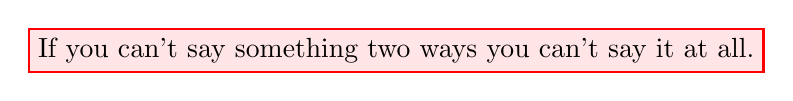
\begin{tikzpicture}
        \node[draw=red, fill=red!10, thick]
            {If you can't say something two ways you can't say it at all.};
    \end{tikzpicture}
\end{center}

This credo may seem odd to linguists, who usually take a strongly realist stance according to which the grammar formalism fully specifies the grammar, even down to notation.
For example, privative (= single-valued) and binary features are regarded as vastly different objects that make very different claims about phonology.
Yet we will see at a later point that they are but two definitions of the same computational object.
% fixme: will we see this?
That does not rule out that one of the two is a more useful way of thinking about phonology, but that is a matter of epistemology rather than ontology.

Returning from our brief methodological excursus, we now have to define bigrams, which in turn will allows us to define bigram grammars.
%
\begin{definition}[Bigrams]
    Given a string $w$ over alphabet $\Sigma$, its \emph{augmented} counterpart $\augmented{w} \is \LeftEdge \stringcat w \stringcat \RightEdge$ is obtained by adding the left and right edge markers $\LeftEdge$ and $\RightEdge$ to $w$, where $\LeftEdge$ and $\RightEdge$ are distinguished symbols not contained in $\Sigma$.
    Furthermore, 
    \(
    \Bigrams(w) \is
        \setof{
            \ngram{ab} \mid \exists u,v \in \Sigma^* \text{ s.t.\ }
                u \stringcat \ngram{ab} \stringcat v = \augmented{w}
        }
    \)
    denotes the set of \emph{bigrams} over $\augmented{w}$, i.e.\ the smallest set that contains all substrings of $\augmented{w}$ that consist of exactly $2$ symbols.
\end{definition}

\begin{definition}[Bigram Grammar]
    A \emph{bigram grammar} $G$ over alphabet $\Sigma$ is a finite set of bigrams over $\Sigma \cup \setof{\LeftEdge, \RightEdge}$.
    If $G$ is a \emph{positive bigram grammar} (denoted $\posG{G}$), then it generates the language
    \(
        L(G) \is \setof{
            w \mid \Bigrams(w) \subseteq G
        }
    \).
    If $G$ is a \emph{negative bigram grammar} (denoted $\negG{G}$), then it generates the language
    \(
        L(G) \is \setof{
            w \mid \Bigrams(w) \cap G = \emptyset
        }
    \).
\end{definition}

With all these definitions under our belt, we can finally move on to producing a new insight: positive and negative bigram grammars are equally powerful.
That is to say, if some language is generated by a positive bigram grammar, then it can also be generated by some negative bigram grammar, and the other way round.

\begin{theorem}
    The class of languages that are generated by positive bigram grammars is exactly the class of languages that are generated by negative bigram grammars.
    \label{thm:SL_PosNegEquivalence}
\end{theorem}
%
In order to show that this theorem is indeed correct, we establish two simpler propositions --- called lemmata --- which jointly imply the theorem.

\begin{lemma}
    For every positive bigram grammar there is a negative bigram grammar that generates the same language.
    \label{lem:SL_Pos2Neg}
\end{lemma}
%
\begin{proof}
    Let $\posG{G}$ be a positive bigram grammar. 
    We show that $\negG{\complementof{G}}$ defines the same language as $\posG{G}$, where $\complementof{G}$ consists of all bigrams over $\Sigma \cup \setof{\LeftEdge, \RightEdge}$ that are not contained by $G$.

    Pick some arbitrary string $w \in L(\posG{G})$. 
    By definition, every bigram of $w$ is a member of $G$, which immediately implies that no element of $\Bigrams(w)$ is contained in $\complementof{G}$.
    But if none of the bigrams of $w$ belong to $\complementof{G}$, then $\Bigrams(w) \cap \complementof{G} = \emptyset$, wherefore $w \in L(\negG{\complementof{G}})$.
    Since $w$ was arbitrary, this result holds for every string generated by $\posG{G}$, establishing $L(\posG{G}) \subseteq L(\negG{\complementof{G}})$.

    The same argument can be applied in the other direction to show $L(\posG{G}) \supseteq L(\negG{\complementof{G}})$, wherefore $L(\posG{G}) = L(\negG{\complementof{G}})$.
\end{proof}
%
This is a so-called \emph{constructive} proof: we do not just show that an equivalent negative bigram grammar exists, we also explain how this grammar can be constructed from the positive bigram grammar.
Constructive proofs are the most useful kind of proof because they provide procedures and strategies that can be implemented and run automatically.

In the case at hand, all we have to do in order to construct an equivalent negative bigram grammar is to take the set-theoretic complement of the positive bigram grammar.
After all, the set of all bigrams over $\Sigma$ is given by $\Sigma \times \Sigma$, and the positive bigram grammar $\posG(G)$ is some subset thereof (\emph{modulo} edge markers, which are treated as part of $\Sigma$ here to avoid notational clutter).
Bigrams that belong to $G$ may occur in a string, bigrams that do not must not.
So the bigrams not belonging to $G$ are the illicit bigrams, which means those are exactly the bigrams the equivalent negative bigram grammar must contain.
In one sentence: taking the complement of $G$ is like taking its negation, and the switch from a positive grammar to a negative one undoes this negation.

So now we know that the negative bigram grammars are at least as powerful as the positive bigram grammars since the latter can be translated into the former.
It only remains for us to show that the same holds in the other direction.

\begin{lemma}
    For every negative bigram grammar there is a positive bigram grammar that generates the same language.
\end{lemma}
%
\begin{proof}
    Left as an exercise to the reader.
\end{proof}
%
Figure~\ref{fig:SL_Proof} gives a pictorial representation of the implications used in these proofs.
%
\begin{figure}
\centering
\begin{tikzpicture}[
    every node/.style = {rounded corners},
    positive/.style = {draw=blue!75,fill=blue!25},
    negative/.style = {draw=red!75,fill=red!25}%
    ]
    \node[positive] (pos-member) at (0,0) {$w \in L(\posG{G})$};
    \node[positive] (subset) [below=of pos-member] {$\Bigrams(w) \subseteq G$};
    \node[negative] (disjoint) [right=5em of subset] {$\Bigrams(w) \cap \complementof{G} = \emptyset$};
    \node[negative] (neg-member) [above=of disjoint] {$w \in L(\negG{\complementof{G}})$};

    \foreach \Source/\Target in {%
        pos-member/subset,
        subset/disjoint,
        disjoint/neg-member%
        }
        \draw[<->] (\Source) to (\Target);
\end{tikzpicture}

\caption{Reasoning chain for the equivalence of positive and negative bigram grammars}
\label{fig:SL_Proof}
\end{figure}

\subsection{The How and Why of Proofs}

Proofs are a difficult art at every level of expertise.
For the beginner, the biggest challenge is often to sort out their train of thought and present it in a clear manner: where do I start, and how do I proceed from there step by step to reach the conclusion?

There are no clear-cut rules here, but it is often helpful to break up the problem into smaller ones, as we did with Thm.~\ref{thm:SL_PosNegEquivalence}.
If two sets $A$ and $B$ need to be shown to be equivalent, one can first prove $A \subseteq B$ and then $B \subseteq A$.
And a statement of the form ``$\phi$ iff $\psi$'' can be broken up into ``$\phi$ entails $\psi$'' and ``$\psi$ entails $\phi$''.
We will encounter several basic proof techniques throughout the course (proof by induction, indirect proofs), but don't worry too much about specific techniques for now.
Instead, make sure to work through the proofs we discuss multiple times until you understand how they work.
Always try to answer the following questions for yourself:

\begin{itemize}
    \item Why is the initial assumption valid?
    \item How does each conclusion follow from the previous one?
    \item Why does the final conclusion show that the theorem\slash lemma is correct?
\end{itemize}

You may wonder why we need proofs in the first place.
Linguists don't work with proofs yet they have discovered a lot of interesting things about language.
Programmers don't have much use for proofs either.
There's several answers, the simplest one being that some questions can only be addressed conclusively via proofs.
Consider the following alternative to the proof of Lem.~\ref{lem:SL_Pos2Neg}: we could have implemented the translation procedure from positive to negative grammars and then tested it on a large sample of positive bigram grammars (at least several thousand).
Eventually the program would have told us that the negative grammars generate the same string languages as their positive counterparts.
So if the conversion works correctly on every single one of thousands of positive bigram grammars, isn't that enough to posit that positive and negative bigram grammars are interchangeable?

The answer is No.
First of all, checking that two grammars generate the same language is hardly trivial if both languages are infinite (we can't just compare all their respective members).
More importantly, though, the thousands of test grammars may accidentally share a special property that is essential for the correctness of the conversion.
This is a real risk if all those test grammars were automatically generated by a script because true randomness is very hard to achieve with computers, if not impossible.
While experiments and simulations have their place --- they are a valid last resort where proofs are hard to come by --- a proof is always the preferred solution where possible.

Proofs are preferred not only because they are safe from the pitfalls of simulations, but also because they provide genuine insight.
In fact, proofs are often more important and enlightening than the theorems they establish.
Testing the correctness of the bigram conversion via automated experiments could at best show us whether the procedure is correct (if there's only finitely many cases to test), but it does not tell us \textbf{why}.
A proof is an explicit record of how certain properties entail others.
In the case at hand, it is the close connection between set-theoretic complementation and the switch from positive to negative grammars that does all the work.
Notice all the properties of bigram grammars that the proof does not depend on: that bigrams are strings, that bigrams consist of exactly two symbols, and that bigram grammars are finite. 
Yet these properties necessarily hold during any test procedure, so we would not be able to tell which one of them is a prerequisite for the correctness of the conversion.
Thanks to the proof, we know which properties matter, which in turn might come in handy in the study of other formalisms.

In a few lines, a proof can establish unassailable truths, show us why they hold, but also save us hours of work compared to running simulations.
So even though you may initially find them hard and time consuming, proofs are actually the tool of choice for the lazy scientist.


\section{Linguistic Evaluation}
The bigram grammar model improves on the list phonology model in various respects.
Variation across languages is now much more restricted because phonology is just a collection of highly local constraints (negative bigram grammars) or permissions (positive bigram grammars).
Bigram grammars also account for linguistic creativity, i.e.\ that speakers can form new words according to the rules of their own language, and that they recognize whether nonce words are well-formed.
As a consequence, they do not predict that the lexicon is finite, either.
Whether the lexicon is finite or infinite is immaterial for bigram grammars since they determine well-formedness in a compositional manner.
As long as each word is finite, its grammaticality can easily be determined via a bigram scanner.

Bigram grammars do still exhibit egalitarianism.
Since a grammar is a list of bigrams, all these bigrams should have the same status and there should be no distictions between easy and difficult processes.
For example, we have seen that the language $(\String{ab})^+$ can be generated by a bigram language.
If we identify $a$ with C and $b$ with V, we get the word template for languages that only allow CV syllables.
Clearly we could just as well have mapped $a$ to V and $b$ to C, generating a language where all words consist of VC syllables.
While many languages can have VC syllables, all languages with VC syllables also allow for CV syllables.
This implicational universal is completely unexpected if phonology is just a bigram grammar.

Isolationism is also a problem as processes still cannot apply across words.
For \emph{phone bill}, the phonological representation is presumably something like \LeftEdge\textipa{foUn}\RightEdge\LeftEdge\textipa{bIl}\RightEdge.
Since \textipa{n} and \textipa{b} are not adjacent, a negative bigram grammar with \ngram{nb} does not have the desired result.
This could be fixed with a bigger search domain, though, which also seems to be necessary for slightly less local processes like intervocalic voicing, where we want to block a voiceless sound only if it occurs between two vowels.

Overall bigram grammars are doing very well on a conceptual level and are easy to implement, but they are not expressive enough for English.
In the next chapter we will see how we can keep all their attractive properties while increasing their power to a more adequate level.

% fixme: exercises
    % - do bigram grammars use less memory than list phonology? by how much? under what circustances is this not the case?
    % - convert bigram grammar into matrix format
    % - define useless bigram
    % - show that every positive grammar has multiple equivalent negative grammars; compute their number;
    % - show that every positive grammar has exactly one equivalent negative grammar

% fixme: scanner operates in linear time


\pagestyle{empty}
% \include{./tex/h1}

\end{document}
